\chapter{基于团树传播的精确推断}
\label{chap:pgm-junction-tree}

设备报警以后，诊断程序可能接连询问故障概率、过热概率，以及故障与传感器失灵的联合概率。第~\ref{chap:pgm-elimination}章的变量消除可以分别回答这些问题，但若每次都从原始因子开始，许多局部求和会重复进行。问题不在于这些求和算错了，而在于一次查询产生的中间结果没有被组织成后续查询可以继续使用的形式。

本章把中间因子保存为\term{消息}（message）：一张只保留边界变量、汇总边界一侧全部贡献的函数表。树结构使这种汇总特别直接，因为删除一条边就能把计算分成两部分。一般图没有这样的边界划分，需要先把相互依赖的变量组合成团，再用满足特定交集条件的树连接这些团。构造是否保留了正确边界、传播是否汇总了完整贡献、查询是否正确使用缓存，是精确性的三个不同问题。

除特别说明外，本章讨论有限离散变量，因子非负且取有限值。记变量节点集合为$V$，$X_i$的状态集合为$\mathcal{X}_i$，$\bm{x}_A$表示$A\subseteq V$上各变量的一组取值。模型参数在推断期间固定，不在消息传播中重新估计。以下求和都是对所标变量的全部状态求和，空乘积约定为$1$。

\section{从变量消除到消息传递}
\label{sec:pgm-junction-tree-from-elimination}

沿用设备故障模型，以二元变量$F,H,A,S$分别表示故障、过热、报警和传感器失灵，其联合分布为
\begin{equation}
  p(f,h,a,s)=p(f)p(h\mid f)p(s)p(a\mid h,s).
  \label{eq:pgm-junction-tree-device}
\end{equation}
这里$p(F=1)=0.1$、$p(S=1)=0.05$，且$p(H=1\mid F=0)=0.1$、$p(H=1\mid F=1)=0.8$。报警条件表见表~\ref{tab:pgm-junction-tree-alarm-cpt}，其余二元概率用$1$减去表中对应值求得。这些参数是人工教学设置，不是设备实测统计。

\begin{table}[htbp]
  \centering
  \begin{tabular}{ccc}
    \toprule
    $h$ & $s$ & $p(A=1\mid h,s)$\\
    \midrule
    $0$ & $0$ & $0.01$\\
    $1$ & $0$ & $0.90$\\
    $0$ & $1$ & $0.70$\\
    $1$ & $1$ & $0.99$\\
    \bottomrule
  \end{tabular}
  \caption{贯穿本章的报警条件概率。$S=1$表示传感器失灵，既可能在不过热时触发报警，也可能与过热同时出现。}
  \label{tab:pgm-junction-tree-alarm-cpt}
\end{table}

观察$A=1$后，为查询$F$而消去$S$，得到
\begin{equation}
  u(h)=\sum_s p(s)p(A=1\mid h,s),
  \qquad (u(0),u(1))=(0.0445,0.9045).
  \label{eq:pgm-junction-tree-boundary-likelihood}
\end{equation}
这个中间因子并非只对查询$F$有用。只要模型参数和报警证据不变，$u(h)$就始终概括传感器与报警对$H$的贡献；计算过热后验时可以直接复用它。另一方面，从故障侧消去$F$得到
\begin{equation}
  v(h)=\sum_f p(f)p(h\mid f),
  \qquad (v(0),v(1))=(0.83,0.17).
  \label{eq:pgm-junction-tree-boundary-prior}
\end{equation}
这张表不依赖报警证据。两侧结果相乘，便有$p(h,A=1)=u(h)v(h)$。一次局部消元因此可以服务于多个查询，也可以在另一侧证据改变以后继续使用。

普通的单次变量消除常在中间因子完成用途后将其丢弃；变量消除本身并不禁止缓存。消息传递进一步规定缓存的作用域、依赖方向和更新规则，使程序知道哪些结果可以共享。图~\ref{fig:pgm-junction-tree-factor-cut}中的因子图是一棵树，切断$H$与报警因子之间的边后，左右两侧只通过$H$的取值联系。固定$h$，各侧可以独立消去内部变量，再把结果相乘。消息就是这种以边界取值为输入的局部计算结果，而不是一个节点向另一个节点传送的单个概率。

\begin{figure}[htbp]
  \centering
  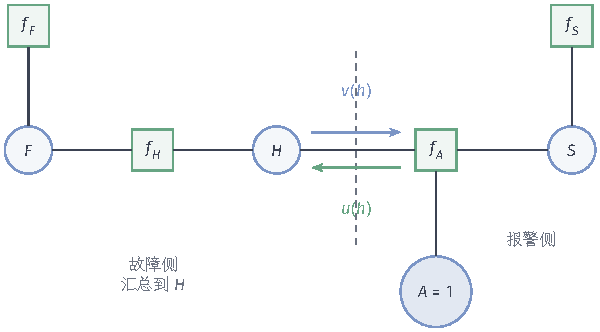
\includegraphics[width=\linewidth]{figures/03-models/03-probabilistic-graphical-models/tikz/pgm-junction-tree-factor-cut/figure.pdf}
  \caption{报警模型的树状因子图。圆表示变量，方框表示因子；$A=1$作为变量处的证据。虚线切断$H$与$f_A$之间的边，蓝色与绿色箭头分别表示两侧汇总得到的$v(h)$和$u(h)$，不是原有向图的因果箭头。}
  \label{fig:pgm-junction-tree-factor-cut}
\end{figure}

这种计算也属于动态规划：对子问题按边界状态制表，较大的子问题只读取相邻子问题的结果。树保证每一侧的贡献有明确归属。若直接在有环图上传播，同一个因子可能沿不同路径回到原处；此时上述互不重叠的子问题解释不再自动成立。

\section{树结构上的消息传递}
\label{sec:pgm-junction-tree-tree-messages}

把局部汇总写成统一公式，需要分清变量节点和因子节点的职责。设因子索引集为$\mathcal{F}$，$f_\alpha$的作用域为$D_\alpha\subseteq V$。每个变量至少属于一个因子；没有实际约束的变量可以添加一个恒为$1$的一元因子。用$\ell_i(x_i)$记录变量处的证据，未观测时取$1$，观测$X_i=e_i$时取指示函数$\mathbf{1}\{x_i=e_i\}$。将全部证据记为$\bm{e}$，定义
\begin{equation}
  \begin{aligned}
    q_{\bm{e}}(\bm{x})
      &=\prod_{\alpha\in\mathcal{F}}f_\alpha(\bm{x}_{D_\alpha})
        \prod_{i\in V}\ell_i(x_i),\\
    Z_{\bm{e}}&=\sum_{\bm{x}}q_{\bm{e}}(\bm{x}),\qquad
    p(\bm{x}\mid\bm{e})=\frac{q_{\bm{e}}(\bm{x})}{Z_{\bm{e}}}.
  \end{aligned}
  \label{eq:pgm-junction-tree-evidence-weight}
\end{equation}
条件分布要求$Z_{\bm{e}}>0$。这里保留了被观测变量，其后验质量集中在观测值上，便于在证据更新时沿用同一张图。若原模型未归一化，其无证据配分函数记为$Z_0$，硬证据的概率为$Z_{\bm{e}}/Z_0$，不能直接把$Z_{\bm{e}}$称为证据概率。

\subsection{和积消息}
\label{sec:pgm-junction-tree-sum-product}

设因子图连通且无环，$N(i)$为变量$i$的相邻因子集合，$N(\alpha)=D_\alpha$为因子$\alpha$的相邻变量集合。\term{和积消息}（sum-product message）用乘法汇合不同分支，再用求和消去不需要传出的变量。变量到因子、因子到变量分别有
\begin{equation}
  m_{i\to\alpha}(x_i)
    =\ell_i(x_i)
      \prod_{\beta\in N(i)\setminus\{\alpha\}}
      m_{\beta\to i}(x_i),
  \label{eq:pgm-junction-tree-variable-message}
\end{equation}
\begin{equation}
  m_{\alpha\to i}(x_i)
    =\sum_{\bm{x}_{D_\alpha\setminus\{i\}}}
      f_\alpha(\bm{x}_{D_\alpha})
      \prod_{j\in D_\alpha\setminus\{i\}}
      m_{j\to\alpha}(x_j).
  \label{eq:pgm-junction-tree-factor-message}
\end{equation}
变量节点只代表同一个$x_i$，所以它将自身证据与其他分支的贡献逐项相乘，不消去$x_i$。因子节点连接多个变量；固定接收方的$x_i$以后，它将其他变量的状态逐一加总，输出仍是一张关于$x_i$的表。

为什么乘积必须排除接收方？切断边$(i,\alpha)$后，$m_{i\to\alpha}$只应包含$i$所在一侧的因子；来自$\alpha$的消息已经汇总了另一侧。若将它乘回去，另一侧的贡献就会被重复计入。对于式~\eqref{eq:pgm-junction-tree-factor-message}，删除$\alpha$后，各邻接变量所在分支互不相交。固定这些邻接变量，分支内部求和可以分别进行，再由分配律提到$f_\alpha$旁边。这就推导出局部更新式，而不是仅凭图形猜测一个递推关系。

在报警例中，令$f_F=p(f)$、$f_H=p(h\mid f)$、$f_S=p(s)$、$f_A=p(a\mid h,s)$。叶侧先得到$m_{F\to f_H}(f)=p(f)$与$m_{S\to f_A}(s)=p(s)$，观测变量发送$m_{A\to f_A}(a)=\mathbf{1}\{a=1\}$。于是
\[
  \begin{aligned}
    m_{f_H\to H}(h)&=\sum_f p(h\mid f)p(f)=v(h),\\
    m_{f_A\to H}(h)&=\sum_{a,s}p(a\mid h,s)
       \mathbf{1}\{a=1\}p(s)=u(h).
  \end{aligned}
\]
因$H$没有自身证据，$m_{H\to f_A}=v$、$m_{H\to f_H}=u$。从两个方向读取同一条边上的消息，读到的是两侧不同的贡献，并非同一条件概率的两种写法。因子图上的这种局部和积规则统一了树上多种动态规划算法\scite{pgm-overview-kschischang2001}

\subsection{消息调度与边缘恢复}
\label{sec:pgm-junction-tree-scheduling}

消息公式还规定了计算顺序：节点向某个邻居发送消息之前，需要收到所有其他邻居的消息。任选一个变量节点作为根，按从叶到根的顺序执行\term{收集}（collect），即把各分支贡献汇总到根。叶变量只发送$\ell_i$，叶因子只发送自己的一元函数。根得到全部入站消息后，再沿从根到叶的顺序执行\term{分发}（distribute），把各节点尚缺少的另一侧贡献传下去。

若因子图有$M$条边，完整传播发送$2M$条有向消息，每个方向恰好一次。树上不存在需要反复迭代等待收敛的问题：收集阶段的依赖按深度递减，分发阶段的依赖按深度递增，都有确定的终止顺序。如果只查询根的边缘，收集已经足够；分发的收益是让其余节点也拥有完整的入站信息。

传播完成后，定义未归一化的局部汇总
\begin{equation}
  \begin{aligned}
    B_i(x_i)&=\ell_i(x_i)\prod_{\alpha\in N(i)}
       m_{\alpha\to i}(x_i),\\
    B_\alpha(\bm{x}_{D_\alpha})
      &=f_\alpha(\bm{x}_{D_\alpha})
        \prod_{j\in D_\alpha}m_{j\to\alpha}(x_j).
  \end{aligned}
  \label{eq:pgm-junction-tree-factor-beliefs}
\end{equation}
以$i$或$\alpha$为中心切开树，所有分支恰好覆盖全图的其余因子，故$B_i=\sum_{\bm{x}_{V\setminus\{i\}}}q_{\bm{e}}$，$B_\alpha=\sum_{\bm{x}_{V\setminus D_\alpha}}q_{\bm{e}}$。两者分别除以$Z_{\bm{e}}$就是相应后验边缘。若变量$i,j$同属$D_\alpha$，对$B_\alpha$中的其他变量求和便能得到$p(x_i,x_j\mid\bm{e})$。对成对因子图，这正是原模型一条边两端变量的联合边缘；因子图自身是二部图，不存在变量节点直接相连的边。

报警例的$H$处给出
\begin{equation}
  (B_H(0),B_H(1))=(0.036935,0.153765),
  \qquad Z_{\bm{e}}=0.19070.
  \label{eq:pgm-junction-tree-alarm-normalizer}
\end{equation}
因此$p(H=1\mid A=1)\approx0.806319$。继续向故障侧分发，$m_{f_H\to F}(f)=\sum_h p(h\mid f)u(h)$，得到$(0.1305,0.7325)$；乘$p(f)$以后便恢复$p(F=1\mid A=1)=0.07325/0.19070\approx0.384111$。

以上等式保留了消息的原始尺度。实际计算中可将一条非零消息整体除以正数，避免很小的权重连乘导致下溢；局部结果再归一化后仍给出相同边缘。但是，经过独立缩放的$B_i$之和不再自动等于$Z_{\bm{e}}$。若需要证据概率，必须同步保存缩放常数并恢复尺度。全零消息不能归一化；它表明该侧所有边界状态都无法与证据相容，需要继续报告零证据权重，而不是任意填入均匀分布。

\subsection{最大积消息}
\label{sec:pgm-junction-tree-max-product}

若目标从“各状态共有多少概率质量”改为“哪一组完整状态权重最大”，求和必须改成最大化。\term{最大积消息}（max-product message）保存边界给定时一侧子树能够达到的最大权重。以$\nu$区别于和积消息，其更新为
\begin{equation}
  \begin{aligned}
    \nu_{i\to\alpha}(x_i)
      &=\ell_i(x_i)\prod_{\beta\in N(i)\setminus\{\alpha\}}
         \nu_{\beta\to i}(x_i),\\
    \nu_{\alpha\to i}(x_i)
      &=\max_{\bm{x}_{D_\alpha\setminus\{i\}}}
         f_\alpha(\bm{x}_{D_\alpha})
         \prod_{j\in D_\alpha\setminus\{i\}}
         \nu_{j\to\alpha}(x_j).
  \end{aligned}
  \label{eq:pgm-junction-tree-factor-max}
\end{equation}
因子非负，才可以在不同分支间使用$\max_{\bm{y},\bm{z}}g(\bm{y})h(\bm{z})=(\max_{\bm{y}}g)(\max_{\bm{z}}h)$。消息只记录最大值还不够；计算$\nu_{\alpha\to i}(x_i)$时，还应为每个$x_i$存储一组达到最大值的$\bm{x}_{D_\alpha\setminus\{i\}}$，称为\term{回溯记录}（backpointer），即根据边界状态找回子问题最优选择的表。

完整的入站最大积消息相乘得到$\widehat{B}_i(x_i)=\ell_i(x_i)\prod_{\alpha\in N(i)}\nu_{\alpha\to i}(x_i)$，它是固定$x_i$以后全图能够达到的最大权重，称为\term{最大边缘}（max-marginal）。它保留的是每个$x_i$下最优配置的权重，而概率边缘累加所有配置的权重，二者不能互相替代。

收集结束后，在根处最大化自身证据与全部入站消息的乘积，确定根状态。随后逐层读取回溯记录：已知父变量状态，就确定相邻因子另一侧各变量的状态，再向更深的分支继续。若最优选择不唯一，可以按固定顺序保存其中一组，但必须沿同一套条件选择回溯。不能让每个变量独立取其最大边缘状态，因为不同位置的任意平局选择可能拼不成一组相容解。例如两个二元变量只有$(0,0)$、$(1,1)$权重为$1$，其余权重为零，则两个位置的最大边缘都对$0,1$平局；各自任意选择可能拼出权重为零的$(0,1)$。

以$H$为根，故障侧的最大积汇总为
\[
  \begin{aligned}
    \nu_{f_H\to H}(0)&=\max(0.9\times0.9,\;0.1\times0.2)=0.81,\\
    \nu_{f_H\to H}(1)&=\max(0.9\times0.1,\;0.1\times0.8)=0.09.
  \end{aligned}
\]
两种$h$都记录$f=0$。报警侧在$h=0$时比较$0.95\times0.01$与$0.05\times0.70$，得$0.035$并记录$s=1$；在$h=1$时比较$0.95\times0.90$与$0.05\times0.99$，得$0.855$并记录$s=0$。根处比较$0.81\times0.035=0.02835$与$0.09\times0.855=0.07695$，选$h=1$。回溯得到全部非证据变量的MPE为$(f,h,s)=(0,1,0)$，未归一化权重为$0.07695$。这里的最大积消息与式~\eqref{eq:pgm-junction-tree-boundary-prior}、式~\eqref{eq:pgm-junction-tree-boundary-likelihood}的和积消息数值不同，不能混用。

当树退化为隐状态链时，设隐状态为$Z_t$，观测为$X_t=x_t$，最大积收集变成
\[
  \delta_t(z_t)=p(x_t\mid z_t)
    \max_{z_{t-1}}\{\delta_{t-1}(z_{t-1})p(z_t\mid z_{t-1})\}.
\]
以$\delta_1(z_1)=p(z_1)p(x_1\mid z_1)$初始化，保存每个$z_t$对应的最优前驱，再从末端回溯，就是Viterbi动态规划。第~\ref{sec:pgm-dynamic-discrete}节将把它用于离散时序模型。这里求的是全部隐状态的联合最优解；只对一部分变量求最优、对其余变量求和的边缘MAP仍受第~\ref{sec:pgm-elimination-map}节的运算顺序约束。

\section{团树的构造}
\label{sec:pgm-junction-tree-construction}

树状因子图允许沿单变量边界汇总，一般因子图却可能含环。要保持精确性，可以让一条消息同时保留多个边界变量，将环内必须共同处理的变量放进同一个计算节点。\term{团树}（junction tree）就是这样一棵以变量团为节点的树：节点是变量集合而不是原图中的单个变量，边表示相邻团的交集而不是原变量图中的边。相邻团可以重叠，但重叠方式必须保证每个变量的信息沿树连续传递。

图~\ref{fig:pgm-junction-tree-triangulation}先给出从含环原图到可复用消息的完整路线。原图指出哪些变量直接共同进入局部因子，却不能沿一条边切成互不重叠的子问题；消元与填充把新产生的依赖记录为弦，避免后续消元遗漏共同作用域；极大团把必须共同处理的变量收进局部计算节点；团树再以团交集作为两侧共享的边界；分配团势并沿每条树边发送两个方向的消息以后，两侧消元结果便能被后续查询复用。图中的每一步都改变计算组织方式，但不额外乘入因子，也不改变原分布。

\begin{figure*}[htbp]
  \centering
  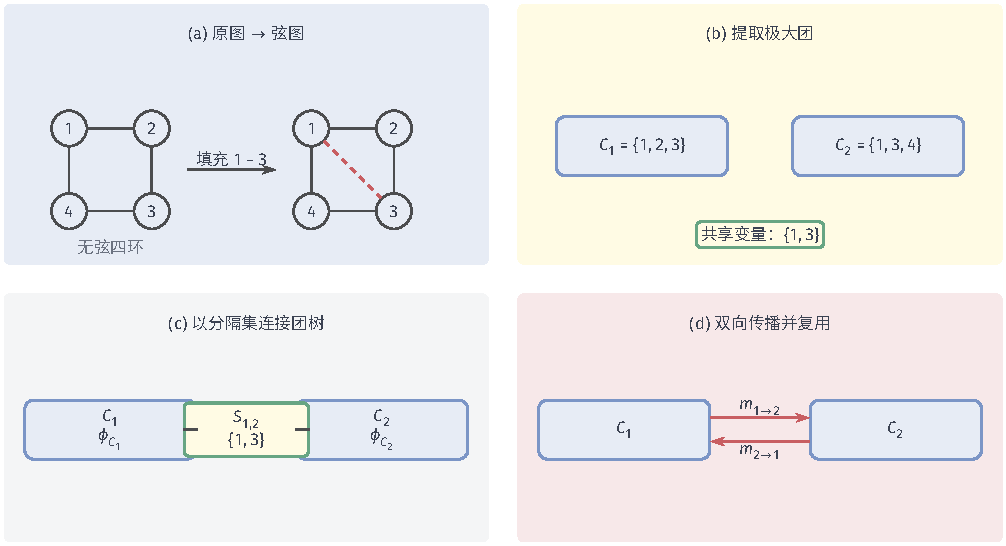
\includegraphics[width=\linewidth]{figures/03-models/03-probabilistic-graphical-models/tikz/pgm-junction-tree-triangulation/figure.pdf}
  \caption{团树编译与传播总览。四个面板按两行两列展开：四环先通过填充边$1-3$变为弦图，再提取极大团$C_1=\{1,2,3\}$与$C_2=\{1,3,4\}$；分隔集$S_{1,2}=\{1,3\}$明确标出两团共享状态，最后用双向消息汇总树边两侧的贡献。团树的节点和边属于计算结构，不是把原变量图改画成树。}
  \label{fig:pgm-junction-tree-triangulation}
\end{figure*}

\subsection{从原图到弦图}
\label{sec:pgm-junction-tree-chordalization}

团应当容纳原始因子的整个作用域。对于有向图，条件因子$p(x_i\mid\bm{x}_{\operatorname{pa}(i)})$同时涉及节点$i$及其全部父节点，因此先连接共同子节点的父节点，再去掉箭头，得到道德图。这里使用的是承载全部因子的整体道德图，不是为了检验某一次条件独立查询而取出的祖先子图。报警模型由此增加$H-S$边，得到团$\{F,H\}$和$\{H,A,S\}$。

对于无向模型，因子作用域本来就应包含在团中；若输入是因子图，则将每个作用域内的变量两两相连，得到相应的变量交互图。接下来按一个选定的消元顺序操作：消去节点时，把它尚未消去的邻居全部连接起来，再移除该节点。将过程中新增的填充边保留在原节点集合上，就得到\term{三角化}（triangulation），也称弦化；结果是一张每个长度至少为$4$的环都有弦的图。

选顺序时，可沿用第~\ref{sec:pgm-elimination-complexity}节的最小度与最小填充启发式：前者少留邻居，后者少添邻居之间缺失的边。填充并不近似掉被消变量的作用，而是把这种作用转存到邻居的共同因子上。每步都保留这个边界子问题的完整汇总，后续才有足够信息继续消元；顺序不同改变的是表格大小，不是合法精确计算的答案。

为什么这个构造产生弦图？在所得图上，所选顺序中每个节点的后继邻居已经两两相连，因而它是完美消除序。若还有一个无弦长环，取环上最早被消去的节点，它在环上的两个邻居都尚未消去，必已相连；这条边恰好是该长环的一条弦，与无弦假设矛盾。第~\ref{chap:pgm-representations}章讨论过图转换的表示含义，这里新增边的计算作用是记录消元以后需要共同保留的变量，而不是新增一个概率因子或改变原来的参数。

图~\ref{fig:pgm-junction-tree-triangulation}中的四环$1-2-3-4-1$也说明消元选择如何决定团的大小。先消去$2$，需要添加$1-3$，得到两个极大团$\{1,2,3\}$和$\{1,3,4\}$；先消去$1$则添加$2-4$，得到$\{1,2,4\}$和$\{2,3,4\}$。两者都能承载同一个原始四环分布，但保存的消息分别定义在$\{1,3\}$和$\{2,4\}$上；变量状态数不同时，这两张表的成本可能相差很大。

\subsection{极大团、分隔集与运行交集性质}
\label{sec:pgm-junction-tree-running-intersection}

一个团内部的节点两两相连；\term{极大团}（maximal clique）是不能再加入其他节点而仍保持团性质的团。“极大”指不能扩充，不是全图中节点数最多。设极大团集合为$\mathcal{C}$，以它们为节点构造树$\mathcal{T}=(\mathcal{C},\mathcal{E}_{\mathcal{T}})$。边$(C,D)$对应的\term{分隔集}（separator）为$S_{C,D}=C\cap D$，它是消息在两个团之间保留的变量集合。

先看图~\ref{fig:pgm-junction-tree-running-intersection}中的三个团$\{1,2\}$、$\{2,3\}$和$\{3,4\}$。按这个顺序连成链时，含$2$的两个团相邻，含$3$的两个团也相邻，$1,4$则各只出现一次。若把$\{3,4\}$放在中间，含$2$的两端之间就隔着一个不含$2$的团。两种连接都是树，但后一种连接无法沿路径保留同一个$x_2$。

因此，仅让团连成树还不够。如果变量$i$出现在两个团中，它在两团之间的每一步传递都必须被保留。否则，中间某条消息会提前消去$i$，而路径另一端又要求按同一个$i$的状态组合因子，已经丢掉的信息无法恢复。

\begin{definition}[运行交集性质]
  \label{def:pgm-junction-tree-running-intersection}
  团树满足\term{运行交集性质}（running intersection property），是指对任意变量$i$，包含$i$的全部团构成连通子树。等价地，对任意两个团$C,D$，从$C$到$D$的唯一路径上的每个团都包含$C\cap D$。
\end{definition}

两种表述的等价性来自树的唯一路径：若包含$i$的团连通，连接任意两个这样的团的路径只能位于该连通子树内；反之，若所有这些路径都保留$i$，这些团便相互连通。

\begin{figure}[htbp]
  \centering
  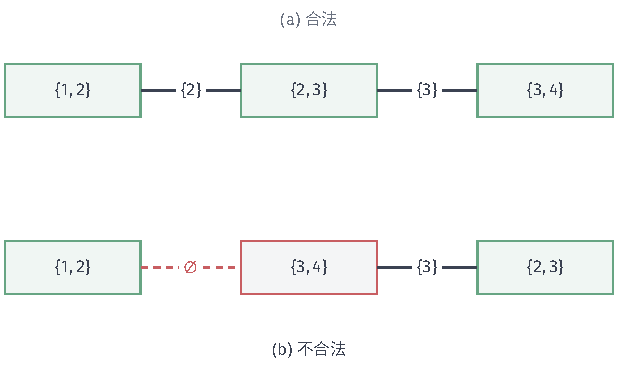
\includegraphics[width=\linewidth]{figures/03-models/03-probabilistic-graphical-models/tikz/pgm-junction-tree-running-intersection/figure.pdf}
  \caption{运行交集检查的是变量是否沿团间路径连续出现。上排$\{1,2\}-\{2,3\}-\{3,4\}$满足要求；下排将$\{3,4\}$放在中间，连接两个含$2$的团时经过了不含$2$的团，即使图形无环也不合法。}
  \label{fig:pgm-junction-tree-running-intersection}
\end{figure}

这个条件可以化为后续证明需要的分隔结论。删除团树边$(C,D)$，令$\mathcal{C}_{C\mid D}$为$C$侧的团集合，并记$U_{C\mid D}=\bigcup_{K\in\mathcal{C}_{C\mid D}}K$。则
\begin{equation}
  U_{C\mid D}\cap U_{D\mid C}=S_{C,D}.
  \label{eq:pgm-junction-tree-cut-intersection}
\end{equation}
包含关系“$\supseteq$”直接来自$C,D$分处两侧。反过来，若$i$出现在两侧各一个团中，连接这两个团的路径必经过边$(C,D)$；运行交集要求$i$同时属于$C,D$，故$i\in S_{C,D}$。这证明两侧共享的变量恰好就是消息所保留的分隔集，不会有另一个共享变量被悄悄消去。

这就允许按分隔集状态做动态规划：固定边界后，两侧各自汇总内部变量，再组合结果。精确性来自分配律和正确的分隔，并非“树宽有限就能高效计算”。有限图的树宽本来就有限；离散稠密表格的成本仍指数依赖所选顺序的诱导宽度，只有团的状态空间可承受时，这种动态规划才实际可行。

运行交集失效时会发生实际数值错误。例如给二元链上的三个团分别分配$\mathbf{1}\{x_1=x_2\}$、$\mathbf{1}\{x_2=x_3\}$和$\mathbf{1}\{x_3=x_4\}$。全局只有全$0$、全$1$两组非零配置，权重和应为$2$。若按图中错误顺序连接，以$\{1,2\}$为根，$\{2,3\}$先向$\{3,4\}$发送常数$1$；$\{3,4\}$再向根发送空分隔集上的标量$2$。根求和得到$2\times2=4$，把两侧本应相同的$x_2$当成了两份可分别求和的变量。树形与局部消息公式都没有错，错在树没有保留原问题要求的共享状态。

\subsection{团树构造与因子分配}
\label{sec:pgm-junction-tree-spanning-tree}

如何从弦图的团中选择正确连接，而不逐棵树尝试运行交集？构造\term{团交图}（clique intersection graph），即将每个极大团作为节点，以交集大小
\[
  w(C,D)=|C\cap D|
\]
作为边权。通常只保留非空交集的边；若原图不连通，可以允许权为$0$的边把各分量连接起来，消息在空分隔集上就是标量。为统一表述，下面把这些零权边也视为候选边。

\begin{theorem}[最大权生成树与团树]
  \label{thm:pgm-junction-tree-maximum-weight}
  设$\mathcal{H}=(V,E)$为非空有限弦图，$\mathcal{C}$为其全部极大团。在以$\mathcal{C}$为节点集合的完全无向图上，对不同团$C,D$定义边权$w(C,D)=|C\cap D|$，其中不相交团之间的边权为$0$。该完全图的一棵生成树满足运行交集性质，当且仅当它是最大权生成树。
\end{theorem}

\begin{proof}
  先说明满足运行交集的树确实存在。取弦图的完美消除序$v_1,\ldots,v_d$，令$N_i^+$为$v_i$的后继邻居，建立集合$K_i=\{v_i\}\cup N_i^+$。若$N_i^+$非空，取其中序号最小的$v_j$，把$K_i$连向$K_j$。由于$N_i^+$是团，$N_i^+\subseteq K_j$。连接方向的序号严格增加，所以没有环；没有后继邻居的节点成为各分量的根。

  若某个$K_i$含$v_k$且$i<k$，其父集合仍含$v_k$，父序号又不大于$k$。不断向父集合移动，最终到达$K_k$。因此包含$v_k$的集合都连向$K_k$，形成连通子树。每个图上的团都包含在某个$K_i$中：取该团最早的节点，其余节点都是它的后继邻居。于是极大团恰好是这些集合中的极大者。对非极大的$K_i$，选择一个包含它的极大集合；连接两者的路径上的每个集合都包含$K_i$，所以可以把$K_i$收缩到路径上的相邻超集中。收缩不破坏任何变量的连通性。重复此操作得到以极大团为节点的树或森林；不同分量之间用空交集连接即可。

  再证明最大权判据。令$k_i$为包含变量$i$的极大团数，$e_i(\mathcal{T})$为候选树中两端都含$i$的边数。这些边构成$k_i$个节点上的森林，故$e_i(\mathcal{T})\leq k_i-1$，等号当且仅当该森林连通。交换求和顺序得到
  \[
    \sum_{(C,D)\in\mathcal{E}_{\mathcal{T}}}|C\cap D|
      =\sum_{i\in V}e_i(\mathcal{T})
      \leq\sum_{i\in V}(k_i-1).
  \]
  已构造出的运行交集树对每个$i$都达到等号，所以上界可以达到。任何最大权树也必须对每个$i$达到等号，否则总权重严格小于该上界；这恰好要求所有含$i$的团连通。反方向同理。
\end{proof}

实际构造时，可以使用最大权版本的Kruskal算法。起初不选任何边，将候选边按交集大小从大到小检查，权重相同时按预定顺序处理。只有当两端的团尚未被已选边连通时，才加入当前边；否则加入它会形成环，应当跳过。直到全部团连通，共选出$|\mathcal{C}|-1$条边，就得到最大权生成树。

复用图~\ref{fig:pgm-junction-tree-running-intersection}中的三个团$\{1,2\}$、$\{2,3\}$和$\{3,4\}$，前两个团的交集为$\{2\}$，后两个团的交集为$\{3\}$，首尾两团的交集为空。三条候选边的权重分别为$1,1,0$。两条权为$1$的边依次连接尚未连通的团，加入后即得到图中上排的链；再加入零权边就会成环，因此不选。

弦图的前提不能省略：例如四环的四个边团无法组成运行交集树，取最大权生成树也不能凭空补足缺失的变量。证明还说明，最大化交集大小的用途是保证变量连通，而不是寻找树宽最小的三角化；三角化已经在构造团交图之前选定。关于分解图、团树及局部计算的系统论述可参见图模型教材\scite{pgm-lauritzen1996}

树确定后，为每个原始因子$f_\alpha$选择且只选择一个覆盖其作用域的团$a(\alpha)$，满足$D_\alpha\subseteq a(\alpha)$。由此定义无证据团势
\begin{equation}
  \phi_C^0(\bm{x}_C)
    =\prod_{\alpha:\,a(\alpha)=C}f_\alpha(\bm{x}_{D_\alpha}),
  \qquad
  \prod_{C\in\mathcal{C}}\phi_C^0
    =\prod_{\alpha\in\mathcal{F}}f_\alpha.
  \label{eq:pgm-junction-tree-factor-assignment}
\end{equation}
没有分到因子的团取恒等势$1$。“能够覆盖”不等于“每个覆盖团都放一份”：若把同一因子复制到两个团，它在乘积中就被平方，模型随之改变。报警例可以取$C_1=\{F,H\}$、$C_2=\{H,A,S\}$，令$\phi_{C_1}^0=p(f)p(h\mid f)$、$\phi_{C_2}^0=p(s)p(a\mid h,s)$，分隔集为$\{H\}$。

不同合法因子分配、不同最大权树和不同三角化都可能保持同一联合分布。它们改变局部表格、消息路由和可复用范围，而不是改变概率答案。团很大但树形简单，仍可能难以计算；这一成本要根据实际状态空间评估。

\section{团树传播}
\label{sec:pgm-junction-tree-propagation}

团树构造解决了共享变量怎样保留的问题。数值传播则将树上的单变量消息扩展为分隔集上的多变量消息。本节采用显式保存双向消息的形式，发送时不需要除以旧消息，因而允许原始因子或证据产生零表项。

\subsection{团势与团间消息}
\label{sec:pgm-junction-tree-clique-messages}

\term{团势}（clique potential）是附在团上的非负函数，用来存储该团负责的原始因子和证据。它不必归一化，也不等于该团的边缘分布。为每个证据因子$\ell_i$选择一个包含$i$的团$h(i)$，令
\begin{equation}
  \phi_C(\bm{x}_C)=\phi_C^0(\bm{x}_C)
    \prod_{i:\,h(i)=C}\ell_i(x_i).
  \label{eq:pgm-junction-tree-local-evidence}
\end{equation}
于是$\prod_C\phi_C=q_{\bm{e}}$。也可以吸收作用于多个变量的似然函数，但必须由某个团完整覆盖它的作用域，并明确该函数代表什么观测机制。每条证据信息只分配一次；重复乘入一般软证据会重复计数，而不只是改变记录方式。

记$N_{\mathcal{T}}(C)$为团$C$的邻居集合。图~\ref{fig:pgm-junction-tree-message}把一条消息拆成可见的输入、消元和输出：发送$C\to D$时，先将团势$\phi_C$与除$D$外全部邻居的入站消息相乘，再消去只属于发送团的变量$C\setminus S_{C,D}$，输出表只保留分隔集$S_{C,D}$中的变量。反向消息执行同一操作，但汇总的是$D$侧贡献；两个方向都完成后，相邻团才能在共享变量上校准。

\begin{figure*}[htbp]
  \centering
  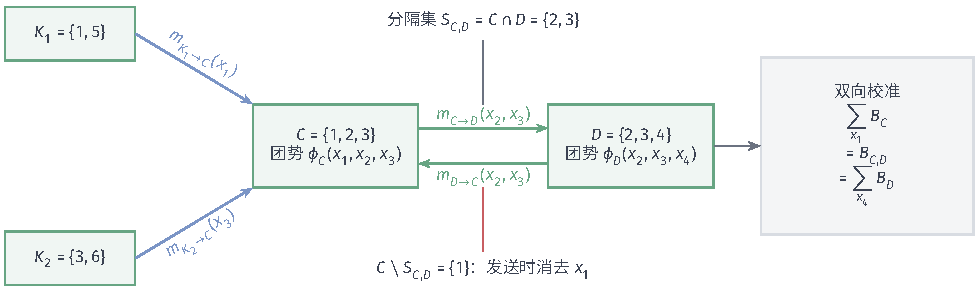
\includegraphics[width=\linewidth]{figures/03-models/03-probabilistic-graphical-models/tikz/pgm-junction-tree-message/figure.pdf}
  \caption{团间消息的组成与双向校准。蓝色箭头是$C$收到的入站消息，团势与这些消息相乘后，对$C\setminus S_{C,D}=\{1\}$中的$x_1$求和，得到定义在分隔集$\{2,3\}$上的$m_{C\to D}$；发送时排除接收方$D$的入站消息。绿色双向箭头分别汇总树边两侧的贡献，收集与分发都完成后，两个团消去非共享变量所得的表均等于分隔集势$B_{C,D}$。}
  \label{fig:pgm-junction-tree-message}
\end{figure*}

将图中的操作写成公式，有
\begin{equation}
  m_{C\to D}(\bm{x}_{S_{C,D}})
    =\sum_{\bm{x}_{C\setminus S_{C,D}}}
      \phi_C(\bm{x}_C)
      \prod_{K\in N_{\mathcal{T}}(C)\setminus\{D\}}
        m_{K\to C}(\bm{x}_{S_{K,C}}).
  \label{eq:pgm-junction-tree-clique-message}
\end{equation}
各函数按相同变量的取值对齐，较小作用域的函数在其余坐标上重复使用。发送消息不修改$\phi_C$；否则下一次发送时可能把已包含在入站消息中的贡献再次乘入。

为了区分局部输入与全局汇总，定义
\begin{equation}
  \begin{aligned}
    B_C(\bm{x}_C)
      &=\phi_C(\bm{x}_C)
        \prod_{K\in N_{\mathcal{T}}(C)}
          m_{K\to C}(\bm{x}_{S_{K,C}}),\\
    B_{C,D}(\bm{x}_{S_{C,D}})
      &=m_{C\to D}(\bm{x}_{S_{C,D}})
        m_{D\to C}(\bm{x}_{S_{C,D}}).
  \end{aligned}
  \label{eq:pgm-junction-tree-clique-separator-beliefs}
\end{equation}
$B_C$称为团的汇总势；$B_{C,D}$是本章采用的\term{分隔集势}（separator potential），汇合边两侧对分隔集的贡献。它由两条消息计算，不是另一个需要乘入原模型的因子。不同边即使具有相同的变量交集，也分别保存自己的双向消息和分隔集势。

在报警例中，把$\ell_A(a)=\mathbf{1}\{a=1\}$放在$C_2$，两个团势为
\[
  \begin{aligned}
    \phi_{C_1}(f,h)&=p(f)p(h\mid f),\\
    \phi_{C_2}(h,a,s)&=p(s)p(a\mid h,s)\ell_A(a).
  \end{aligned}
\]
两团都是叶端，所以没有额外入站消息：
\begin{equation}
  \begin{aligned}
    m_{C_1\to C_2}(h)&=\sum_f p(f)p(h\mid f)=v(h),\\
    m_{C_2\to C_1}(h)&=\sum_{a,s}p(s)p(a\mid h,s)\ell_A(a)=u(h).
  \end{aligned}
  \label{eq:pgm-junction-tree-device-clique-messages}
\end{equation}
它们与树状因子图中的两侧汇总完全相同。更大的团树只是把原来数步消元合并为一次团间消息，不会引入新的概率运算。

\subsection{收集、分发与校准}
\label{sec:pgm-junction-tree-calibration}

以团$R$为根，叶团向父团收集消息；一个非叶团收到所有子团消息后，再发送自己的父向消息。根拥有全部入站消息时，开始向每个子团分发。算法~\ref{alg:pgm-junction-tree-calibrate}给出完整调度。消息尚未计算不能与“恒为$1$”混为一谈；只有公式中的空乘积才自然等于$1$。

\begin{algorithm}[团树上的和积校准]
  \label{alg:pgm-junction-tree-calibrate}
  \begin{algorithmic}[1]
    \Require 满足运行交集的团树、局部势$\{\phi_C\}$、根$R$
    \Ensure 全部双向消息、汇总势$\{B_C,B_{C,D}\}$和$Z_{\bm{e}}$
    \State 将树定根，记录每个非根团的父团
    \For{按后序遍历访问的非根团$C$}
      \State 按式~\eqref{eq:pgm-junction-tree-clique-message}发送$C$到父团的消息
    \EndFor
    \For{按先序遍历访问的团$C$}
      \For{$C$的每个子团$D$}
        \State 按式~\eqref{eq:pgm-junction-tree-clique-message}发送$C\to D$
      \EndFor
    \EndFor
    \State 按式~\eqref{eq:pgm-junction-tree-clique-separator-beliefs}形成汇总势
    \State 计算$Z_{\bm{e}}=\sum_{\bm{x}_R}B_R(\bm{x}_R)$
    \If{$Z_{\bm{e}}=0$}
      \State 报告证据与模型不相容，不输出条件概率
    \Else
      \State 令$b_C=B_C/Z_{\bm{e}}$、$b_{C,D}=B_{C,D}/Z_{\bm{e}}$
    \EndIf
  \end{algorithmic}
\end{algorithm}

完整传播后，各团不仅吸收了全部证据，还会对共享变量给出相同的分布。\term{校准}（calibration）在这里指这种重叠边缘的一致性，不是分类器置信度与经验频率之间的预测校准。它要求相邻团把非共享变量消去以后，得到相同的分隔集势，图~\ref{fig:pgm-junction-tree-message}右侧的等式正是这项检查。

这个一致性可以直接由消息公式证明。对边$(C,D)$，$m_{D\to C}$只依赖$S_{C,D}$，因此能提出关于$C\setminus S_{C,D}$的求和号：
\begin{equation}
  \begin{aligned}
    &\sum_{\bm{x}_{C\setminus S_{C,D}}}B_C(\bm{x}_C)\\
      &\quad=m_{D\to C}
        \sum_{\bm{x}_{C\setminus S_{C,D}}}
          \phi_C\prod_{K\in N_{\mathcal{T}}(C)\setminus\{D\}}m_{K\to C}\\
      &\quad=m_{D\to C}m_{C\to D}=B_{C,D}.
  \end{aligned}
  \label{eq:pgm-junction-tree-local-calibration}
\end{equation}
从$D$侧作同样的计算也得到$B_{C,D}$。所以两个团对分隔集的汇总完全一致。第~\ref{sec:pgm-junction-tree-correctness}节将进一步证明$B_C$确实是$q_{\bm{e}}$的边缘；仅有“相邻表一致”还不足以断定它们对应最初输入的模型。

报警例的双向消息与分隔集势见表~\ref{tab:pgm-junction-tree-calibrated-separator}。每一行固定同一个$h$，两条消息相乘就是两团共同认可的$H$权重；列和$0.19070$给出证据概率。

\begin{table}[htbp]
  \centering
  \begin{tabular}{cccc}
    \toprule
    $h$ & $m_{C_1\to C_2}(h)$ & $m_{C_2\to C_1}(h)$ & $B_{C_1,C_2}(h)$\\
    \midrule
    $0$ & $0.83$ & $0.0445$ & $0.036935$\\
    $1$ & $0.17$ & $0.9045$ & $0.153765$\\
    \bottomrule
  \end{tabular}
  \caption{报警证据下的双向消息和分隔集势。只有最后一列是$H$与证据的联合权重；单独一条消息不必是归一化分布。}
  \label{tab:pgm-junction-tree-calibrated-separator}
\end{table}

还可以逐项检查两个团的汇总势。以下第一张表按$f$分行、$h$分列，第二张按$h$分行、$s$分列；第二张只列$a=1$的切片，$a=0$切片全为零：
\begin{equation}
  \begin{aligned}
    \bigl[B_{C_1}(f,h)\bigr]_{f,h}
      &=\begin{pmatrix}
          0.036045&0.081405\\
          0.000890&0.072360
        \end{pmatrix},\\
    \bigl[B_{C_2}(h,1,s)\bigr]_{h,s}
      &=\begin{pmatrix}
          0.007885&0.029050\\
          0.145350&0.008415
        \end{pmatrix}.
  \end{aligned}
  \label{eq:pgm-junction-tree-device-calibrated-tables}
\end{equation}
第一张表按列求和，第二张表按行求和，都得到$(0.036935,0.153765)$。各表的总和也都等于$0.19070$。这同时核对了因子分配、消息方向与校准；不必另做一次完整枚举才知道两个团的重叠部分是否一致。

若消息已独立缩放，应分别将团汇总势归一化，再比较它们在分隔集上的概率边缘；不应要求那些带有不同任意尺度的原始表直接相等。构造可复用的局部表示并吸收、传播证据，是经典精确图模型推断的核心思路\scite{pgm-overview-lauritzen1988}

\subsection{查询与证据更新}
\label{sec:pgm-junction-tree-queries-updates}

校准以后，若查询集合$Q$包含于某个团$C$，答案就是
\begin{equation}
  p(\bm{x}_Q\mid\bm{e})
    =\sum_{\bm{x}_{C\setminus Q}}b_C(\bm{x}_C).
  \label{eq:pgm-junction-tree-covered-query}
\end{equation}
无需重新传播消息，但仍要完成团表内部的边缘化，并写出所需输出。在报警例中，$F,H$由$C_1$覆盖，$H,S$由$C_2$覆盖；分别消去另一个变量即可得到$p(F=1\mid A=1)\approx0.384111$与$p(S=1\mid A=1)\approx0.196460$。

查询$\{F,S\}$却没有被任何一个团共同覆盖。虽然两个团的汇总势都已经正确，它们各自都包含了全图证据；直接相乘会重复使用重叠部分的信息。在本例中，正确拼接为
\begin{equation}
  p(f,s\mid A=1)
    =\frac{1}{Z_{\bm{e}}}
      \sum_h
       \frac{B_{C_1}(f,h)B_{C_2}(h,1,s)}
            {B_{C_1,C_2}(h)}.
  \label{eq:pgm-junction-tree-cross-clique-device}
\end{equation}
两个分母值在本例中均为正。以$(f,s)=(0,0)$为例，归一化之前的两项为
\[
  \begin{aligned}
    &\frac{0.036045\times0.007885}{0.036935}
     +\frac{0.081405\times0.145350}{0.153765}\\
    &=0.007695+0.076950=0.084645.
  \end{aligned}
\]
式中除去一个分隔集势，恰好撤掉重复的$H$权重。四组结果见表~\ref{tab:pgm-junction-tree-cross-query}，与直接消去$H$得到的联合表一致。

\begin{table}[htbp]
  \centering
  \begin{tabular}{cccc}
    \toprule
    $f$ & $s$ & $p(f,s,A=1)$ & $p(f,s\mid A=1)$\\
    \midrule
    $0$ & $0$ & $0.084645$ & $0.443865$\\
    $0$ & $1$ & $0.032805$ & $0.172024$\\
    $1$ & $0$ & $0.068590$ & $0.359675$\\
    $1$ & $1$ & $0.004660$ & $0.024436$\\
    \bottomrule
  \end{tabular}
  \caption{没有单团覆盖的查询$\{F,S\}$。末列为四舍五入值；联合表不能由两个一元后验相乘得到，也不能由未经分隔集修正的团势乘积得到。}
  \label{tab:pgm-junction-tree-cross-query}
\end{table}

遗漏分隔集修正并不是只差一个全局常数。若错误地将两个团汇总势直接相乘，再消去$H$，会得到
\[
  \widetilde{q}(f,s)=\sum_h B_{C_1}(f,h)B_{C_2}(h,1,s).
\]
对$\widetilde{q}$整体归一化，所得故障概率约为$0.446232$，而正确值是$0.384111$。额外乘入的$B_{C_1,C_2}(h)$随$h$改变，归一化无法消去这种状态相关的偏差。

一般的跨团查询可以只处理覆盖查询变量的连通子树。为每个查询变量选择一个包含它的团，将连接这些团的子树的团集合记为$\mathcal{H}\subseteq\mathcal{C}$，并令$W=\bigcup_{C\in\mathcal{H}}C$。外部各分支已有消息，将它们吸收到子树内的局部势：
\begin{equation}
  \begin{aligned}
    \widetilde{\phi}_C
      &=\phi_C
        \prod_{D\in N_{\mathcal{T}}(C)\setminus\mathcal{H}}m_{D\to C},\\
    g_Q(\bm{x}_Q)
      &=\sum_{\bm{x}_{W\setminus Q}}
         \prod_{C\in\mathcal{H}}\widetilde{\phi}_C(\bm{x}_C),\\
    p(\bm{x}_Q\mid\bm{e})&=g_Q(\bm{x}_Q)/Z_{\bm{e}}.
  \end{aligned}
  \label{eq:pgm-junction-tree-subtree-query}
\end{equation}
运行交集保证每个外部分支只通过对应分隔集与子树连接，因此这些入站消息已经完成对$V\setminus W$的求和。子树内部再执行变量消除即可，不需要显式展开$W$上的全部联合表。这种形式复用了校准时的消息，且没有除法，在含零势时也成立。

如果只保存了校准后的团边缘和分隔集边缘，也可以在它们的正支持上使用
\begin{equation}
  p(\bm{x}_W\mid\bm{e})
    =\frac{\prod_{C\in\mathcal{H}}b_C(\bm{x}_C)}
           {\prod_{(C,D)\in\mathcal{E}_{\mathcal{H}}}
                b_{C,D}(\bm{x}_{S_{C,D}})},
  \label{eq:pgm-junction-tree-calibrated-factorization}
\end{equation}
再消去$W\setminus Q$，其中$\mathcal{E}_{\mathcal{H}}$为子树内部的边集。将式~\eqref{eq:pgm-junction-tree-clique-separator-beliefs}代入可见，每条内部边的两条消息恰好各被约去一次，留下$\prod_C\widetilde{\phi}_C$；分子比分母多一个归一化因子，留下$1/Z_{\bm{e}}$。这就给出了该拼接公式的依据，而不是假定团边缘相互独立。

当某个分隔集状态概率为零时，与它一致的完整配置也只能有零概率，不能在该处机械计算$0/0$。可直接使用无除法的式~\eqref{eq:pgm-junction-tree-subtree-query}；也可给子树定根，仅在分隔集概率为正的状态上形成$b_C/b_{C,D}$作为条件表，从零概率父状态到达的分支整体记为零。式~\eqref{eq:pgm-junction-tree-calibrated-factorization}据此按支持集延拓。若只需几个边缘，这比拼出全联合表节省计算；若要求输出很大的联合表，输出成本本身仍不能避免。

MPE查询必须使用另一套最大积消息。对团间消息中的求和换成最大化，得到$\nu_{C\to D}$，并记录
\begin{equation}
  \rho_{C\to D}(\bm{x}_{S_{C,D}})
    \in\argmax_{\bm{x}_{C\setminus S_{C,D}}}
       \left\{\phi_C
          \prod_{K\in N_{\mathcal{T}}(C)\setminus\{D\}}\nu_{K\to C}\right\}.
  \label{eq:pgm-junction-tree-clique-backpointer}
\end{equation}
在根团选择最佳配置，再按已确定的分隔集状态向外回溯。运行交集保证与先前已赋值变量的重叠全部位于分隔集中，所以回溯不会为同一变量给出冲突赋值。若只求一组MPE，最大积收集加回溯已经足够；若需各团的最大边缘，可以另做双向最大积校准。它的重叠一致性使用最大化，不是求和，汇总势也不再表示概率边缘。已完成的和积消息不能在查询时临时“改成最大化”使用；即使根据和积校准结果重建了联合分布，仍需重新完成所需最大化和回溯运算。

证据更新与更换查询不同，它可能让缓存失效。设$\mathcal{D}$为局部势发生变化的团集合。根据消息的一侧子树含义，$m_{C\to D}$只依赖$\mathcal{C}_{C\mid D}$侧的局部势，因此
\begin{equation}
  \mathcal{C}_{C\mid D}\cap\mathcal{D}=\varnothing
  \quad\Longrightarrow\quad
  m_{C\to D}\text{可原样复用}.
  \label{eq:pgm-junction-tree-update-dependency}
\end{equation}
反之，只要源侧包含变化团，就应将消息视为可能失效；特殊数值可能使它恰好不变，但仅凭图结构不能作此保证。式~\eqref{eq:pgm-junction-tree-update-dependency}描述的是依赖范围，而不是宣称每次证据变化都一定改变其中每个数值。

若只有$C_0$变化，以它为根，则所有指向$C_0$的消息都不依赖$\phi_{C_0}$，可以保留；只需沿远离$C_0$的方向重新分发，总计重算每条边的一个方向。图~\ref{fig:pgm-junction-tree-evidence-update}展示了这一点。虽然只改了一个局部输入，全树团边缘都可能变化。若只查询团$C_q$覆盖的变量，只需将变化沿$C_0$到$C_q$的唯一路径传过去，其他分支向该路径发来的消息仍有效；尚未刷新的团边缘应保持失效标记，不能当成新证据下的答案。多个团同时变化时，对每个消息应用同一源侧判据，某些边的两个方向都可能需要重算。

\begin{figure}[htbp]
  \centering
  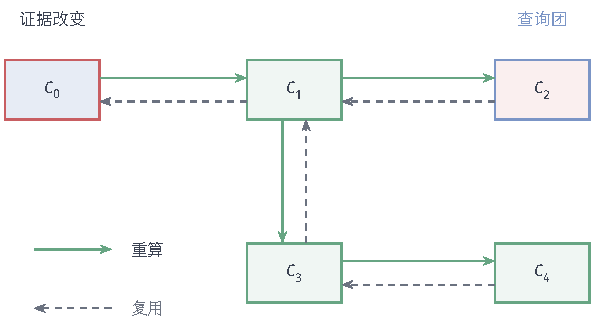
\includegraphics[width=\linewidth]{figures/03-models/03-probabilistic-graphical-models/tikz/pgm-junction-tree-evidence-update/figure.pdf}
  \caption{仅$C_0$的局部势改变时的更新方向。实线箭头沿远离$C_0$的方向传播新贡献，反向虚线箭头表示仍可复用的消息；团节点只画名称，具体变量集合须满足运行交集。查询$C_2$时只需更新路径$C_0-C_1-C_2$，其他团的旧边缘不因路径更新而自动全部有效。}
  \label{fig:pgm-junction-tree-evidence-update}
\end{figure}

在报警例中，新加入$S=0$时只改变$C_2$。保留$m_{C_1\to C_2}=(0.83,0.17)$，重算反向消息为$(0.0095,0.855)$，得到$Z_{\bm{e}}=p(A=1,S=0)=0.153235$和$p(F=1\mid A=1,S=0)=0.068590/0.153235\approx0.447613$。若从只有$A=1$的情形改为$A=0$，反向消息变为$(0.9555,0.0955)$，证据概率为$0.80930$，故障后验为$0.02675/0.80930\approx0.033053$。两种更新都没有理由重算故障侧的先验汇总。

证据撤回不能简单用新指示函数除以旧指示函数。旧硬证据可能把一整片表项置零，除法无法恢复原数值。应保留$\phi_C^0$及各条当前证据，按式~\eqref{eq:pgm-junction-tree-local-evidence}重建受影响的局部势，再按依赖方向重算消息；缩放常数也属于缓存状态，需要同步更新。若曾为某一证据取值删去变量或裁剪图结构，撤回时还须恢复相应结构。

固定团树能够处理被现有团覆盖的证据因子或原有因子的数值变化；它不保证覆盖新加入的多变量似然或结构边。新作用域若不在任何现有团中，就需要重新组织因子、扩大团或重新三角化，不能只把新函数塞入一个不覆盖它的团。相互矛盾的硬证据使$Z_{\bm{e}}=0$时，消息代数仍能计算零权重，但条件后验没有定义。证据更新的正确性必须同时检查缓存依赖、因子覆盖和归一化条件。

\section{算法分析}
\label{sec:pgm-junction-tree-analysis}

\subsection{正确性与校准}
\label{sec:pgm-junction-tree-correctness}

局部校准等式只说明两个邻团彼此一致。为了证明它们一致地表示了输入模型，还要把一条消息与明确的全局求和联系起来。以下定理给出这种联系，也为跨团查询和证据更新提供依据。

\begin{theorem}[子树消息与团边缘]
  \label{thm:pgm-junction-tree-correctness}
  设$V$为有限变量索引集，每个$X_i$的状态空间有限非空；$\mathcal{T}=(\mathcal{C},\mathcal{E}_{\mathcal T})$是以$V$的子集为团节点、满足$\bigcup_{C\in\mathcal C}C=V$和运行交集性质的有限树。有限个取有限非负值的因子与证据因子恰好各分配给一个覆盖其作用域的团，所得团势为$\phi_C$，并记未归一化目标$q_{\bm e}(\bm{x})=\prod_{C\in\mathcal C}\phi_C(\bm{x}_C)$。对边$(C,D)$，令$S_{C,D}=C\cap D$；删除该边后，记$C$侧的团集合为$\mathcal{C}_{C\mid D}$，并令$U_{C\mid D}=\bigcup_{K\in\mathcal{C}_{C\mid D}}K$。若按式~\eqref{eq:pgm-junction-tree-clique-message}完成全部未缩放和积消息，则对每条有向边$C\to D$，
  \begin{equation}
    m_{C\to D}(\bm{x}_{S_{C,D}})
      =\sum_{\bm{x}_{U_{C\mid D}\setminus S_{C,D}}}
         \prod_{K\in\mathcal{C}_{C\mid D}}\phi_K(\bm{x}_K).
    \label{eq:pgm-junction-tree-subtree-invariant}
  \end{equation}
  完整传播后，定义
  \[
    \begin{aligned}
      B_C(\bm{x}_C)&\mathrel{:=}
        \phi_C(\bm{x}_C)
        \prod_{K\in N_{\mathcal{T}}(C)}
          m_{K\to C}(\bm{x}_{S_{K,C}}),\\
      B_{C,D}(\bm{x}_{S_{C,D}})&\mathrel{:=}
        m_{C\to D}(\bm{x}_{S_{C,D}})
        m_{D\to C}(\bm{x}_{S_{C,D}}),\\
      Z_{\bm e}&\mathrel{:=}
        \sum_{\bm{x}_V}q_{\bm e}(\bm{x}).
    \end{aligned}
  \]
  则对任意团$C$及边$(C,D)$，
  \begin{equation}
    \begin{aligned}
      B_C(\bm{x}_C)
        &=\sum_{\bm{x}_{V\setminus C}}q_{\bm{e}}(\bm{x}),\\
      B_{C,D}(\bm{x}_{S_{C,D}})
        &=\sum_{\bm{x}_{V\setminus S_{C,D}}}q_{\bm{e}}(\bm{x}).
    \end{aligned}
    \label{eq:pgm-junction-tree-true-marginals}
  \end{equation}
  若$Z_{\bm e}>0$，则$B_C/Z_{\bm e}$与$B_{C,D}/Z_{\bm e}$分别为相应的后验团边缘和后验分隔集边缘。
\end{theorem}

\begin{proof}
  对$\mathcal{C}_{C\mid D}$中的团数归纳。若这一侧只有叶团$C$，式~\eqref{eq:pgm-junction-tree-subtree-invariant}就是$\sum_{\bm{x}_{C\setminus S_{C,D}}}\phi_C$，与叶消息公式相同。

  对一般的$C$，删去$C$以后，除$D$侧外的每个邻团$K$带来一个分支。记其内部变量集合为$R_K=U_{K\mid C}\setminus S_{K,C}$。运行交集保证$R_K$与$C$不相交：若变量同时在$K$侧某团和$C$中出现，路径经过$K$，它就必须属于$S_{K,C}$。不同$R_K$也不相交，否则连接两分支中该变量的路径经过$C$，再次迫使它属于$C$，与内部变量的定义矛盾。

  因而$U_{C\mid D}\setminus S_{C,D}$可以拆为$C\setminus S_{C,D}$和这些互不相交的$R_K$。固定$\bm{x}_C$，分支中的求和可独立进行；由归纳假设，每个分支的结果恰好是$m_{K\to C}$。有限求和的分配律给出
  \[
    \begin{aligned}
      &\sum_{\bm{x}_{U_{C\mid D}\setminus S_{C,D}}}
         \prod_{L\in\mathcal{C}_{C\mid D}}\phi_L\\
      &\quad=\sum_{\bm{x}_{C\setminus S_{C,D}}}\phi_C
         \prod_{K\in N_{\mathcal{T}}(C)\setminus\{D\}}
          \left[
            \sum_{\bm{x}_{R_K}}
              \prod_{L\in\mathcal{C}_{K\mid C}}\phi_L
          \right]\\
      &\quad=\sum_{\bm{x}_{C\setminus S_{C,D}}}\phi_C
         \prod_{K\in N_{\mathcal{T}}(C)\setminus\{D\}}m_{K\to C}.
    \end{aligned}
  \]
  最后一行正是消息更新式，归纳完成。

  对任意团$C$，将所有邻接分支都纳入上述分解。各分支内部变量互不重叠，且与$C$合起来覆盖$V$；各局部势的乘积又恰为$q_{\bm{e}}$。因此先消去分支内部变量，所得结果为$\phi_C\prod_K m_{K\to C}=B_C$，证明了第一个边缘等式。再把$C\setminus S_{C,D}$消去，利用式~\eqref{eq:pgm-junction-tree-local-calibration}得到$B_{C,D}$，证明第二个等式。两者的全状态求和均为$Z_{\bm{e}}$，在其为正时除以它即可。
\end{proof}

证明中的关键不是“树上的计算天然正确”，而是运行交集使各分支的内部变量真正互不重叠，唯一分配使因子既不遗漏也不重复。分隔集保存全部共享变量，分配律才允许把全局求和拆成局部消息。任意构造一组相邻一致的表，最多说明它们可在合适的树上拼成某个分布；若不检查这些表与原始因子乘积的关系，就不能据此认定它们是所求模型的边缘。

同样的归纳把求和换成最大化，就得到最大积消息的子树最优值含义，因为非负乘法对独立变量组上的最大化仍满足所需分配律。回溯进一步保证取得该值的配置能够拼接：给定分隔集，记录的局部最优选择达到发送消息的数值；沿树展开时，已赋值部分与未展开分支的交集只在分隔集中。逐步代入这些选择，最终联合权重等于根处最大值。若根处最大值为零，则不存在正权重的相容配置，不能将任意零权重配置报告成有定义的条件MPE。

这些证明不要求所有表项严格为正，严格正性只会简化涉及比值的重构。推广到连续变量时，求和应换成积分，并要求存在适当密度、归一化常数有限且为正，以及各局部积分能够精确完成。非负函数可借助Tonelli定理交换积分，但这个代数事实不保证一般函数的积分存在闭式表达，更不能把连续观测的单点指示函数直接照搬为离散硬证据。

\subsection{与变量消除的关系}
\label{sec:pgm-junction-tree-ve-relation}

三角化本来就是变量消除产生的图结构记录。消去$v_i$时，把当前涉及它的因子相乘，乘积作用域落在$\{v_i\}\cup N_i^+$内；消去$v_i$后产生的新因子作用在$N_i^+$上。这与定理~\ref{thm:pgm-junction-tree-maximum-weight}证明中集合$K_i$向父集合发送的消息具有相同边界。把各个消元集合保留下来，便得到一种以中间因子为边的计算树。

若将包含在相邻大集合中的非极大集合收缩掉，就得到更紧凑的团树。收缩相当于把数步局部消元合并为一次团间消息。因此，一条极大团之间的消息可能对应一组变量的连续消除，而不一定与单个变量消除步骤一一对应；没有必要强行给每张中间表找一个独立极大团。

反过来，给定一棵团树并选定根，可以从叶团开始消去该团不属于父分隔集的变量。运行交集保证这些变量不会在尚未处理的其他团中出现，所以可以在此时消去。将所得分隔集因子送到父团，再继续处理，恰好得到团树的收集阶段。这说明两种方法使用相同的乘法和边缘化，并拥有相同的正确性依据，只是组织中间结果的方式不同。

报警例中，以$C_1=\{F,H\}$为根，$C_2$中的$A,S$通过指示证据和求和被消去，生成$u(h)$；根再对$H$求和便得到故障查询。以$C_2$为根时，另一方向消去$F$得到$v(h)$。团树把这两个方向的结果同时保存，因此后续查询$F,H,S$的边缘无需各自重走一遍原始消元。

团树的优势应与任务口径一起理解。只问一次、只需一个目标边缘时，合适的变量消除可以及时释放不用的中间表，未必需要全树分发。固定模型上反复读取不同团覆盖的边缘、或在局部修改证据时，保存双向消息才会带来持续复用。变量消除也可以实现缓存；团树提供的是一套可检查的缓存依赖与失效规则，而不是一种绕过消元计算的独立原理\scite{pgm-koller2009}

\subsection{复杂度与适用边界}
\label{sec:pgm-junction-tree-complexity}

消息数量随树边数线性增长，不意味着其算术成本只随原图节点数线性增长。令$k=|\mathcal{C}|$、$r_i=|\mathcal{X}_i|$，定义团与分隔集的表规模
\begin{equation}
  r_C=\prod_{i\in C}r_i,\qquad
  r_{C,D}=\prod_{i\in S_{C,D}}r_i.
  \label{eq:pgm-junction-tree-table-sizes}
\end{equation}
一条$C\to D$消息输出$r_{C,D}$个数，但在通用稠密表格实现中，通常需要遍历$r_C$个团状态，组合局部势和入站消息，再将它们累加到分隔集相应位置。较小的输出表不能消除形成它所需的团内枚举。

记$\deg(C)$为团的度。单独逐条计算$C$的每个出站消息，每条都重新乘所有其他入站消息，会带来$O(\deg(C)^2r_C)$的重复乘法。可以在每个团状态上计算邻居消息值的前缀积、后缀积，以$O(\deg(C))$次乘法得到排除任意一个邻居的乘积，再分别累加到消息表。这个方法也适用于零表项，不需要用“总乘积除以被排除消息”。结合收集与分发调度，完整传播的时间可界为
\begin{equation}
  O\!\left(\sum_{C\in\mathcal{C}}(\deg(C)+1)r_C\right),
  \label{eq:pgm-junction-tree-time}
\end{equation}
这里假设局部势已经建立，因子表索引等基本操作耗时有界；加$1$还计入形成团汇总势的成本。未采用这种复用的实现应如实保留额外度数因子。

保存局部势、团汇总势和两套方向消息，持久内存的量级为
\begin{equation}
  O\!\left(
    \sum_{C\in\mathcal{C}}r_C+
    2\sum_{(C,D)\in\mathcal{E}_{\mathcal{T}}}r_{C,D}
  \right),
  \label{eq:pgm-junction-tree-memory}
\end{equation}
还应另计输入因子、工作缓冲区与最大积回溯记录。前缀积和后缀积可以逐个团状态临时形成，不必把每个邻居的完整团维度副本永久保存。只保留消息而按需重建团边缘也能减少常数开销，但不能消除大团状态空间。

若每个变量至多有$r$个状态，所选三角化的最大团大小为$w+1$，则$r_C\leq r^{w+1}$。利用树上$\sum_C\deg(C)=2(k-1)$，式~\eqref{eq:pgm-junction-tree-time}给出$O(kr^{w+1})$的传播上界；若有$m$个原始因子，按稠密表格建立局部势的保守上界为$O(mr^{w+1})$。不同极大团的分隔集大小至多为$w$，消息表不超过$r^w$，但团势表仍需要$r^{w+1}$项。这里$w$是已选消元顺序的诱导宽度；只有在最优三角化下，它才等于原交互图的树宽。

状态数不同时，只比较团中变量个数也不够。对于图~\ref{fig:pgm-junction-tree-triangulation}的四环，假设$r_1=r_3=10$、$r_2=r_4=2$，两种三角化的开销如表~\ref{tab:pgm-junction-tree-triangulation-cost}。最大团都含三个变量，但团表与分隔集表的规模明显不同。这提示排序启发式还应考虑各变量状态数，而非只数新增边。

\begin{table}[htbp]
  \centering
  \begin{tabular}{cccc}
    \toprule
    填充边 & 极大团 & 各团表项数 & 分隔集表项数\\
    \midrule
    $1-3$ & $\{1,2,3\},\{1,3,4\}$ & $200,\;200$ & $100$\\
    $2-4$ & $\{1,2,4\},\{2,3,4\}$ & $40,\;40$ & $4$\\
    \bottomrule
  \end{tabular}
  \caption{同一四环的两种精确编译。这里比较人工设定的状态空间规模，不比较概率值；两种选择的未加权树宽都为$2$。}
  \label{tab:pgm-junction-tree-triangulation-cost}
\end{table}

指数开销很快会超过缓存带来的收益。一个含$30$个二元变量的团需要$2^{30}$个表项，仅一张双精度表就占$8$\,GiB，尚未计入其他团、消息与工作空间。最大权生成树的选择不能缩小已经形成的极大团；局部证据更新虽然可能只重算一部分消息，最坏情况下仍会把变化传播到全树。非单团覆盖的联合查询还需要额外局部消元，其受限消元顺序和输出表规模也可能远大于单团边缘查询。

这些界针对任意稠密离散势，并非所有函数表示都按状态组合制表。例如高斯势可以通过精度矩阵与一次项表示，积分消息对应块矩阵消元，其开销由矩阵维数和填充控制，而不是$r^{w+1}$。但这种优势依赖函数族在乘法和积分下的闭包；混合分量增长或一般非线性势会破坏简洁表示。不能只因为图被编成一棵树，就把局部积分、最优化或大表枚举都当成常数操作。

团树适合因子作用域固定、编译成本可以摊销、且最大团可容纳的重复推断任务。若树宽或状态空间已经过大，完整精确表格本身无法保存，团树不会通过复用使它突然可行。直接在有环图上迭代消息属于另一条路线，其固定点与误差问题留到第~\ref{sec:pgm-variational-bethe}节；这些近似算法不能继承本章依赖树分隔与运行交集的精确性证明。

\section{本章小结}
\label{sec:pgm-junction-tree-summary}

变量消除产生的中间因子之所以能够复用，是因为它概括的是一侧子问题对边界变量的完整贡献，而不只是某次查询中的临时数值。树状因子图直接提供这种边界；一般图则通过道德化、三角化和团树构造，把需要共同保留的变量放到团与分隔集中。运行交集保证两侧共享的变量没有遗漏，唯一因子分配保证原始乘积没有被改写。

在这些条件下，收集与分发完成对子树贡献的精确汇总。当证据归一化常数$Z_{\bm e}>0$时，校准后的团汇总势$B_C$除以$Z_{\bm e}$，给出真实后验边缘；局部团势$\phi_C$仍保存本团负责的输入因子与证据。被单团覆盖的查询可以局部读取；跨团查询需要利用分隔集修正或已有边界消息继续消元，不能把多个团边缘直接相乘。MPE使用独立的最大积传播与回溯，证据更新则依据每条消息的源侧依赖判断失效，并在撤回硬证据时从原始势恢复信息。

团树没有改变精确推断的局部代数，却把计算结果与依赖关系显式保存下来。因此，固定模型上的多次查询能够共享计算，局部证据变化也能保留不受影响的消息。复用减少的是重复劳动，不是最大团状态空间：树宽、变量状态数和查询输出规模仍决定这条精确路线能走多远。
